\documentclass[11pt,a4paper,oneside]{article}
\usepackage[a4paper,top=2cm,bottom=3cm,left=2cm,right=2cm]{geometry}
\usepackage[T1]{fontenc}
\usepackage[utf8]{inputenc}
\usepackage[italian]{babel}
\usepackage{frontespizio}
\usepackage{graphicx}
\usepackage{subfig}
\usepackage[italian]{varioref}

\begin{document}

%opzione per doppio interlinea
\baselineskip 12pt


%Indice%
\tableofcontents\thispagestyle{empty}\clearpage

\section{Introduzione}
\pagenumbering{arabic}
Il cancro della prostata è uno dei tumori più diffusi nella popolazione maschile e rappresenta circa il 20\% di tutti i tumori diagnosticati nell'uomo: le stime, relative all'anno 2017, parlano di 34.800 nuovi casi l'anno in Italia, ma il rischio che la malattia abbia un esito infausto è basso, soprattutto se si interviene in tempo.
Lo scopo di questo studio è quello di cercare un modello per poter prevedere la diagnosi di un tumore di questo tipo, partendo dai dati fisici del nodulo prostatico, ottenibili da esami poco invasivi, così da poter offrire la possibilità di velocizzare l'intervento in caso di tumore maligno.

\section{Tabella dei dati}
Il dataset è stato recuperato dal sito \emph{https://www.kaggle.com/sajidsaifi/prostate-cancer}. È costituito da 100 campioni relativi a casi di cancri rilevati, per ognuno dei quali si hanno a disposizione le seguenti caratteristiche:
\begin{itemize}
\item \textbf{Diagnosis Result}: indica se il cancro sia stato diagnosticato come benigno (0) o maligno (1)
\item \textbf{Radius}: raggio approssimativo del nodulo
\item \textbf{Texture}: struttura del nodulo (più è disomogeneo più è alta la probabilità che sia maligno)
\item \textbf{Perimeter}: perimetro approssimativo del nodulo
\item \textbf{Area}: area approssimativa del nodulo
\item \textbf{Smoothness}: regolarità del nodulo, quanto il tessuto è liscio
\item \textbf{Compactness}: compattezza del nodulo, calcolata in funzione del volume e della superficie
\item \textbf{Simmetry}: simmetria del nodulo (più il tessuto è asimmetrico più è alto il rischio di malignità)
\item \textbf{Fractal Dimension}: dimensione frattale relativa al nodulo, rapporto che fornisce un indice statistico di complessità (in \%)
\end{itemize}

\begin{figure}[h]
\centering
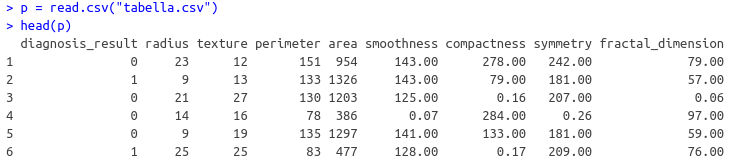
\includegraphics[width=0.7\textwidth]{images/head}
\caption{Prime righe del file \textit{tabella.csv}}
\label{fig:head}
\end{figure}

\section{Analisi dei dati}
Iniziamo l'analisi dei dati, con l'obiettivo di ottenere un modello in grado, se possibile, di classificare ogni caso di tumore come benigno o maligno, basandosi sugli attributi a disposizione.
\subsection{Regressione Logistica}
Proviamo, per prima cosa, una classificazione tramite regressione logistica. Questo metodo si adatta bene al nostro studio perché offre un output dicotomico. Si calcola quindi il modello lineare generalizzato, ponendo come valore di uscita il risultato della diagnosi, per poi procedere con la predizione delle probabilità di appartenenza alla classe $1$ (cancro maligno) e $0$ (cancro benigno).
\begin{verbatim}
> p.glm=glm(diagnosis_result~.,family=binomial,data=p)
> p.glm.pre=predict(p.glm,type="response")
\end{verbatim}
L'accuratezza del modello è molto soddisfacente:
\begin{verbatim}
> sum((p.glm.pre>0.5)==(p$diagnosis_result>0.5))/length(p$diagnosis_result)
[1] 0.89
\end{verbatim}
e questo significa che la nostra classificazione ha senso di esistere. Da notare anche il valore $AIC$, che è molto alto (87\%).
\begin{figure}[ht]
\centering
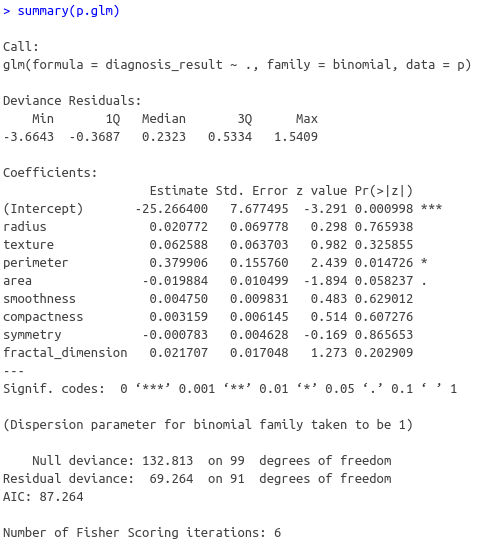
\includegraphics[width=0.4\textwidth]{images/glm}
\caption{Sommario della regressione logistica sui dati}
\label{fig:glm}
\end{figure}
Procediamo, per cui, con l'analisi della matrice di confusione, della curva $ROC$ e dell'area sotto alla curva:
\begin{verbatim}
> mconfmat(p$diagnosis_result,p.glm.pre)
            actual 1 actual 0
predicted 1       59        8
predicted 0        3       30
> p.glm.roc=mroc(p$diagnosis_result,p.glm.pre)
> mroc.plot(p.glm.roc)
> mauc(p.glm.roc)
[1] 0.9210526
\end{verbatim}
Vediamo dalla matrice che i veri positivi, cioè le osservazioni che appartengono alla classe $1$ e sono stati effettivamente classificati come casi maligni, risultano 59 su un totale di 62, e questo risultato è molto buono per il nostro scopo. È, infatti, fondamentale che i casi gravi, per cui è necessario effettuare un rapido intervento, vengano individuati correttamente. Le osservazione relative, invece, a tumori benigni sono state individuate con una percentuale più bassa, dal momento che ne sono state classificate correttamente solo 30 su 38. Si è ottenuto, perciò, un $TNR$ (True Negative Rate) uguale al 79\%, a fronte di un $TPR$ (True Positive Rate) del 95\%.
Andando infine a studiare la curva $ROC$ (fig.~\vref{fig:curveROC}), possiamo confermare quanto trovato nella matrice di confusione: la curva non è perfetta, ma è di molto sopra al tirare a caso (linea rossa tratteggiata). L'area sotto la curva, uguale al 92\% è ulteriore conferma della bontà del nostro modello.

\subsection{Analisi Discriminante Lineare e Quadratica}
Proviamo a effettuare anche un'analisi discriminante, per poter poi confrontare i vari modelli ottenuti e vedere quale è da ritenere migliore per il nostro problema di classificazione.

Effettuiamo, inizialmente, il calcolo del modello lineare e ne valutiamo l'efficacia tramite la predizione:
\begin{verbatim}
> p.lda=lda(diagnosis_result~.,data=p,CV=F)
> p.lda.pre=predict(p.lda)
> p.lda.post=p.lda.pre$posterior[,2] #prob. a posteriori di ottenere 1
> sum((p.lda.post>0.5)==(p$diagnosis_result>0.5))/length(p$diagnosis_result)
[1] 0.86
\end{verbatim}
Otteniamo un'accuratezza dell'86\%, più bassa di tre punti rispetto al modello precedente, ma comunque alta. Procediamo con la valutazione, visualizzando la matrice di confusione e la curva $ROC$ (fig.~\ref{fig:curveROC}):
\begin{verbatim}
> mconfmat(p$diagnosis_result,p.lda.post)
            actual 1 actual 0
predicted 1       57        9
predicted 0        5       29
> p.lda.roc=mroc(p$diagnosis_result,p.lda.post)
> mroc.plot(p.lda.roc)
> mauc(p.lda.roc)
[1] 0.9089559
\end{verbatim}
Possiamo notare che anche nella matrice di confusione viene sottolineata una perdita di accuratezza, poiché si ha un maggior numero di predizioni incorrette rispetto al modello costruito tramite regressione logistica, fatto confermato dalla curva $ROC$, la cui area risulta leggermente minore.

Eseguiamo l'analisi discriminante quadratica, calcolando il modello ed effettuandone la valutazione attraverso gli stessi mezzi:
\begin{verbatim}
> p.qda=qda(diagnosis_result~.,data=p,CV=F)
> p.qda.pre=predict(p.qda)
> p.qda.post=p.qda.pre$posterior[,2]
> sum((p.qda.post>0.5)==(p$diagnosis_result>0.5))/length(p$diagnosis_result)
[1] 0.87
> mconfmat(p$diagnosis_result,p.qda.post)
            actual 1 actual 0
predicted 1       56        7
predicted 0        6       31
> p.qda.roc=mroc(p$diagnosis_result,p.qda.post)
> mroc.plot(p.qda.roc,col="blue")
> mauc(p.qda.roc)
[1] 0.890745
\end{verbatim}
In questo caso, otteniamo un guadagno nell'accuratezza (87\%) in confronto al modello lineare, mentre la curva evidenzia invece un peggioramento del modello: le predizioni sono, infatti, migliori in generale perché il numero di tumori classificati come maligni è più vicino alla realtà (63 rispetto al totale effettivo 62), ma nel particolare si riscontra un maggior numero di falsi positivi e falsi negativi.
\begin{figure}[h]
\centering
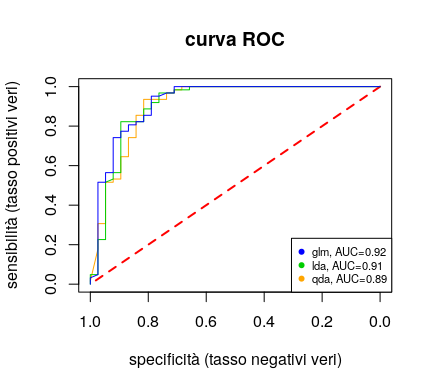
\includegraphics[width=0.5\textwidth]{images/curveROC}
\caption{Curve ROC relative ai tre modelli analizzati}
\label{fig:curveROC}
\end{figure}

\subsection{Conclusioni}
Possiamo concludere che il primo modello, basato sulla regressione logistica, è il più soddisfacente: in particolare, è quello che riesce a classificare il maggior numero di tumori maligni, considerato il caso più critico e quindi più importante da rilevare. Grazie a questa classificazione, possiamo dire che ci sono buone probabilità di poter intervenire in supporto degli esami medici, e velocizzare il processo diagnostico del tumore preso in considerazione, riuscendo a segnalare tempestivamente i casi più gravi considerando le caratteristiche fisiche del tessuto istologico che sono identificabili tramite esami veloci e poco invasivi. È da sottolineare che quest'analisi viene effettuata su un numero relativamente ristretto di osservazioni, per cui sarà interessante portarla avanti aggiungendo dati di altri casi per vedere se l'accuratezza viene mantenuta su larga scala.

\section{Appendice}
Prendendo in considerazione il modello di figura~\vref{fig:glm}, abbiamo analizzato le correlazioni tra gli attributi per cercare di ridurlo mantenendo risultati il più alti possibili. Abbiamo trovato una forte relazione tra $area$ e $perimeter$


\end{document}